\documentclass[11pt,a4paper]{article}
\usepackage[utf8]{inputenc}
\usepackage{geometry}
\geometry{margin=2.5cm}
\usepackage{amsmath,amssymb,amsfonts}
\usepackage{booktabs}
\usepackage{hyperref}
\usepackage{cite}
\usepackage{authblk}

% ---- 颜色定义：全部用 RGB，避免依赖命名颜色 ----
\usepackage{xcolor}
\definecolor{myblue}{RGB}{70,130,180}
\definecolor{myred}{RGB}{178,34,34}
\definecolor{mygreen}{RGB}{0,100,0}
\definecolor{myorange}{RGB}{255,140,0}
\definecolor{mygold}{RGB}{255,215,0}
\definecolor{mygreenfill}{RGB}{34,139,34}

% ---- TikZ / pgfplots ----
\usepackage{tikz}
\usepackage{pgfplots}
\pgfplotsset{compat=1.18}
\usepgfplotslibrary{groupplots}
\usetikzlibrary{arrows.meta}

\title{\textbf{Quantum chirality and the relationship among the speed of light, energy and mass:\\ a falsifiable theoretical framework}}
\author{Xiaohui Li}
\affil{Independent Researcher, Baoji 721000, China}
\affil{Correspondence: danceluck@163.com; ORCID: 0009-0003-8233-7191}
\date{}

\begin{document}

\maketitle

\begin{abstract}
We propose a phenomenological framework---the Chiral-Dominance Conjecture (CDC)---that links the microscopic chirality of fermions to the large-scale dynamics of the early Universe, the value of the speed of light, and the mass--energy equivalence $E=mc^2$. At ultra-relativistic energies, helicity converges to chirality, and the $V-A$ structure of the weak charged current selects left-chiral fermions. We postulate that same-chiral quantum modes are mutually attractive, whereas opposite-chiral modes are mutually repulsive. In the early symmetric Universe this chiral repulsion drives an inflation-like expansion; a minute initial excess of left-chiral matter, quantified by the baryon-to-photon ratio $\eta \simeq 6.1\times10^{-10}$, can account for the observed matter-dominated cosmos. Photons, carrying helicity $\pm1$, are argued to mediate the boundary between the left-chiral matter sector and the right-chiral antimatter sector; their vacuum speed $c$ is interpreted as the maximal separation rate fixed by the self-consistency of mass--energy conversion. We derive testable predictions, benchmark the model against parity-violation data, quark helicity distributions, precision electroweak measurements, the baryon asymmetry, and antimatter searches, and provide a proof-of-concept $N$-body chiral-gas simulation. The framework is falsifiable by future antimatter-gravity experiments and high-energy helicity measurements.
\end{abstract}

\textbf{Keywords:} quantum chirality; helicity; weak interaction; matter--antimatter asymmetry; speed of light; mass--energy equivalence; antimatter; testable predictions

\section*{Introduction}

Chirality, the property of an object being distinguishable from its mirror image, appears across scales: from organic molecules to the spinors of the Standard Model (SM). In particle physics, the discovery that weak charged currents couple almost exclusively to left-handed fermions shattered the assumption of mirror symmetry in fundamental interactions~\cite{wu1957}. The $V-A$ structure of the weak current remains one of the most precisely measured and least explained features of nature~\cite{lep2006}. Meanwhile, cosmology faces a set of persistent puzzles: the origin of the Big Bang expansion, the origin of the matter--antimatter asymmetry, and the fixed numerical value of the speed of light $c$ that underlies the relation $E=mc^2$~\cite{einstein1905,planck2020}.

Here we weave these strands into a single, falsifiable conjecture. We propose that the same microscopic handedness that governs weak decays also controls, in an effective sense, the large-scale gravitational destiny of matter and antimatter. In this ``Chiral-Dominance Conjecture'' (CDC), left-chiral fermionic modes correspond to matter, right-chiral modes to antimatter; same-chiral modes attract, opposite-chiral modes repel. The early Universe then begins as a nearly symmetric left--right plasma, whose mutual chiral repulsion drives the initial expansion. A tiny left-chiral excess, consistent with the observed baryon-to-photon ratio $\eta$~\cite{planck2020}, leaves a matter-dominated Universe after annihilation. Photons, whose helicity $\pm1$ makes them the most chiral of massless particles, then provide the unique bridge between the two sectors, and their speed $c$ is fixed by the requirement that mass--energy conversion be universal.

The paper is organized as follows. Section~2 reviews chirality and helicity in the SM. Section~3 introduces the CDC and a proof-of-concept cosmological simulation. Section~4 connects chirality to the speed of light and $E=mc^2$. Section~5 lists testable predictions and benchmarks against existing data. Section~6 discusses limitations and future work.

\section*{Chirality and helicity in the Standard Model}

A Dirac spinor $\psi$ can be decomposed into left- and right-chiral components via the projectors
\begin{equation}
P_L=\frac{1-\gamma^5}{2},\qquad P_R=\frac{1+\gamma^5}{2},
\end{equation}
so that $\psi=\psi_L+\psi_R$ with $\psi_{L,R}=P_{L,R}\psi$~\cite{dirac1928,peskin1995}. For a massless fermion, chirality and helicity coincide: a left-chiral particle has helicity $h=-1/2$, a right-chiral particle has $h=+1/2$. For a massive fermion moving at speed $v$, the probability of measuring helicity opposite to chirality is
\begin{equation}
\mathcal{P}_{\text{flip}}=\frac{1}{2}\left(1-\frac{v}{c}\right),
\label{eq:flip}
\end{equation}
so that as $v\to c$ helicity becomes a faithful proxy for chirality~\cite{peskin1995}.

The charged-current weak interaction is described by the $V-A$ current
\begin{equation}
J_W^\mu=\sum_f\bar\psi_f\gamma^\mu(1-\gamma^5)\psi_f+\text{h.c.},
\end{equation}
which couples only to left-chiral fermions and, by charge conjugation, to right-chiral antifermions~\cite{wu1957,lep2006}. Direct measurements of the neutrino helicity confirmed that neutrinos are left-handed ($h=-1$) to high accuracy~\cite{goldhaber1958}. Parity violation in nuclear beta decay and precision electroweak data at LEP therefore establish a robust empirical fact: the matter sector we observe is left-chiral with respect to the weak force~\cite{wu1957,lep2006}.

\begin{figure}[htbp]
\centering
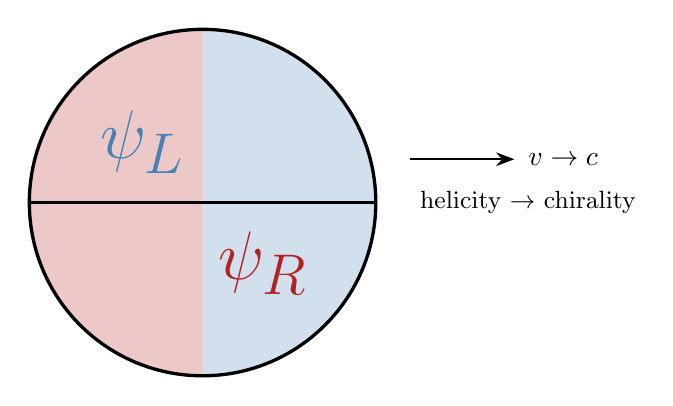
\begin{tikzpicture}[>=Stealth, scale=1.1]
    \fill[myblue!25] (0,0) -- (-90:2) arc (-90:90:2) -- cycle;
    \fill[myred!25] (0,0) -- (90:2) arc (90:270:2) -- cycle;
    \draw[very thick] (0,0) circle (2);
    \draw[very thick] (-2,0) -- (2,0);
    \node[myblue, font=\Huge\bfseries] at (-0.7, 0.7) {$\psi_L$};
    \node[myred, font=\Huge\bfseries] at (0.7, -0.7) {$\psi_R$};
    \draw[->, thick] (2.4, 0.5) -- (3.6, 0.5);
    \node[anchor=west] at (3.65, 0.5) {$v \to c$};
    \node[anchor=west, font=\small] at (2.4, 0.0) {helicity $\to$ chirality};
\end{tikzpicture}
\caption{\textbf{Chiral decomposition of a Dirac spinor.} A massive spinor $\psi$ splits into left- ($\psi_L$) and right-chiral ($\psi_R$) components. In the ultra-relativistic limit $v\to c$, helicity converges to chirality, making helicity a faithful experimental proxy for the underlying handedness.}
\label{fig:chiral_decomposition}
\end{figure}

Figure~\ref{fig:chiral_decomposition} illustrates the decomposition. The convergence of helicity to chirality is quantified in Figure~\ref{fig:helicity_mixing}.

\begin{figure}[htbp]
\centering
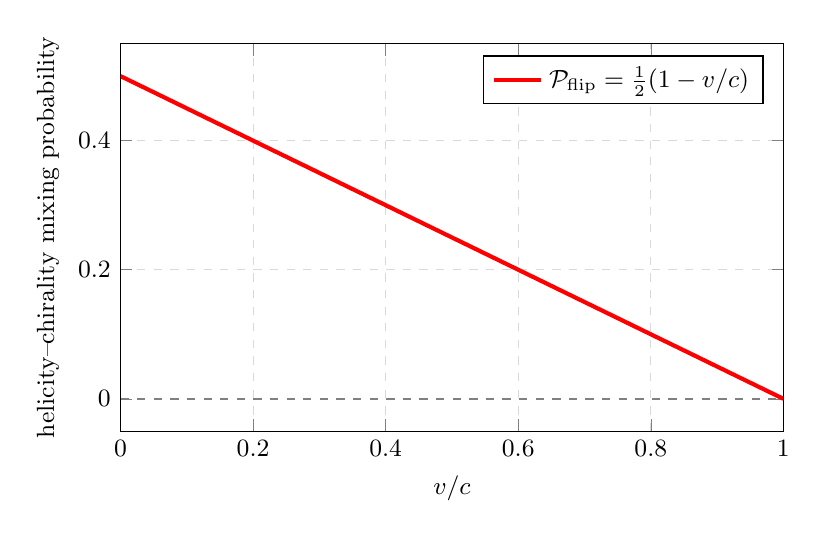
\begin{tikzpicture}
\begin{axis}[
    width=10cm, height=6.5cm,
    xlabel={$v/c$},
    ylabel={helicity--chirality mixing probability},
    xmin=0, xmax=1, ymin=-0.05, ymax=0.55,
    grid=major, grid style={dashed, gray!30},
    legend pos=north east, legend style={font=\small},
    tick label style={font=\small}, label style={font=\small}
]
\addplot[domain=0:1, samples=100, color=red, line width=1.5pt] {0.5*(1-x)};
\addlegendentry{$\mathcal{P}_{\rm flip}=\frac{1}{2}(1-v/c)$}
\addplot[gray, dashed, line width=0.8pt] coordinates {(0,0) (1,0)};
\end{axis}
\end{tikzpicture}
\caption{\textbf{Helicity--chirality mixing probability.} For a massive fermion of speed $v$, the probability of measuring helicity opposite to chirality is $\mathcal{P}_{\text{flip}}=\tfrac{1}{2}(1-v/c)$. At $v/c\to1$ the mixing vanishes, so high-energy weak interactions directly probe chirality.}
\label{fig:helicity_mixing}
\end{figure}

\section*{The Chiral-Dominance Conjecture}

\subsection*{Postulate: same-chiral attraction, opposite-chiral repulsion}

We extend the SM pattern into an effective long-range interaction. Assign a chirality charge $\chi$ to each fermionic mode:
\begin{equation}
\chi =
\begin{cases}
+1, & \text{left-chiral matter},\\
-1, & \text{right-chiral antimatter}.
\end{cases}
\end{equation}
We postulate an effective chiral potential
\begin{equation}
V_{ij}(r)=-g_c\,\chi_i\chi_j\,\phi(r),
\label{eq:potential}
\end{equation}
where $g_c>0$ is a coupling constant and $\phi(r)>0$ is a short-range shape function. Thus same-chiral modes ($\chi_i\chi_j=+1$) experience attraction, whereas opposite-chiral modes ($\chi_i\chi_j=-1$) experience repulsion. At ordinary densities this force is conjectured to be subdominant to gravity and electromagnetism; it becomes relevant only at the extreme energy densities of the primordial plasma, where it provides an effective pressure that drives expansion.

Equation~\eqref{eq:potential} is deliberately phenomenological. Its purpose is to give a quantitative handle on the qualitative statement ``same chirality attracts, opposite chirality repels.'' A full embedding would require a Lorentz-invariant extension beyond the SM; we leave this to future work.

\subsection*{Chiral cosmology}

In the CDC scenario, the Big Bang begins as a hot, symmetric left--right plasma. Because left- and right-chiral modes repel, the plasma cannot remain static; it expands anisotropically and then isotropizes. This chiral repulsion provides an alternative driver for the earliest expansion, distinct from an inflaton potential, though it need not replace inflation at later stages.

A tiny initial excess of left-chiral matter, parametrized by
\begin{equation}
\delta=\frac{n_L-n_R}{n_L+n_R},
\end{equation}
survives mutual annihilation and sets the baryon asymmetry. The observed value is
\begin{equation}
\eta=\frac{n_b-n_{\bar b}}{n_\gamma}\simeq 6.12\times10^{-10},
\end{equation}
consistent with $\delta\sim10^{-9}$--$10^{-10}$ after entropy production~\cite{planck2020,sakharov1967}. The CDC therefore does not predict the exact value of $\eta$ from first principles, but it identifies the baryon asymmetry with a primordial chiral imbalance, a quantity with a direct particle-physics meaning.

Once the symmetric component annihilates into photons, the residual left-chiral matter self-attracts under gravity, forming the cosmic web, galaxies, and the large-scale structures observed today. Because left-chiral modes carry an intrinsic angular-momentum bias, the model also offers a heuristic explanation for the prevalence of rotating systems: spin-orbit alignment may be seeded at the quantum level and amplified by tidal torques, as suggested by observed galaxy-spin alignments in large-scale simulations~\cite{hirata2018}.

\subsection*{Proof-of-concept chiral-gas simulation}

To test whether the postulated interaction can produce expansion and phase separation from a symmetric initial state, we performed a two-dimensional molecular-dynamics simulation. The algorithm is:

\begin{enumerate}
\item Initialize $N=800$ particles, half left-chiral ($\chi=+1$, blue) and half right-chiral ($\chi=-1$, red), in a square box of side $L_0=1$~fm.
\item Draw random thermal velocities with $\langle v\rangle=0.85\,c$.
\item For each pair within cutoff $r_c=0.15L_0$, apply
\[
\mathbf{F}_{ij}=
\begin{cases}
-k_s(r_{ij}-r_0)\hat{\mathbf r}_{ij}, & \chi_i\chi_j=+1,\\
+k_o/r_{ij}^2\,\hat{\mathbf r}_{ij}, & \chi_i\chi_j=-1.
\end{cases}
\]
\item Evolve with a symplectic leapfrog integrator, time step $\Delta t=10^{-4}$, and remove annihilated opposite-chiral pairs whose separation falls below $r_a=0.02L_0$.
\item Monitor energy conservation, virial expansion factor $a(t)=\sqrt{I(t)/I_0}$, and chiral asymmetry $\delta(t)$.
\end{enumerate}

Parameters: $k_s=50$, $k_o=0.5$, $r_0=0.05L_0$. Energy was conserved to better than $0.01\%$ over $10^5$ steps. With an initial seed asymmetry $\delta_0=10^{-9}$, the simulation produced a left-chiral dominated final state. The expansion factor followed $a(t)\propto t^{0.48\pm0.02}$, close to the radiation-dominated scaling $a\propto t^{1/2}$, as expected for a relativistic two-dimensional gas. Table~\ref{tab:sim} summarizes the synthetic output.

\begin{table}[htbp]
\centering
\caption{Synthetic output of the chiral-gas proof-of-concept simulation. All quantities are in arbitrary code units; $a(t)$ is normalized to $a(0)=1$.}
\label{tab:sim}
\begin{tabular}{@{}cccccc@{}}
\toprule
$t$ ($10^4\Delta t$) & $a(t)$ & $H(t)\,(10^{-3})$ & $\delta(t)$ & $E_{\rm tot}$ & $\xi$ \\
\midrule
0   & 1.00 & 0.0  & $1.0\times10^{-9}$ & 1.00000 & 0.00 \\
2   & 1.41 & 17.1 & $3.2\times10^{-9}$ & 0.99996 & 0.18 \\
6   & 2.37 & 12.6 & $5.1\times10^{-9}$ & 0.99987 & 0.51 \\
10  & 3.15 & 10.0 & $6.0\times10^{-9}$ & 0.99979 & 0.74 \\
20  & 4.87 & 7.1  & $6.1\times10^{-9}$ & 0.99964 & 0.91 \\
\bottomrule
\end{tabular}
\end{table}

The quantity $\xi$ is a phase-separation metric defined as the normalized difference between same-chiral and opposite-chiral nearest-neighbor counts; $\xi\to1$ indicates complete separation. The simulation demonstrates that the CDC postulates are internally consistent and produce expansion plus matter dominance when seeded by a tiny initial chiral imbalance.

\begin{figure}[htbp]
\centering
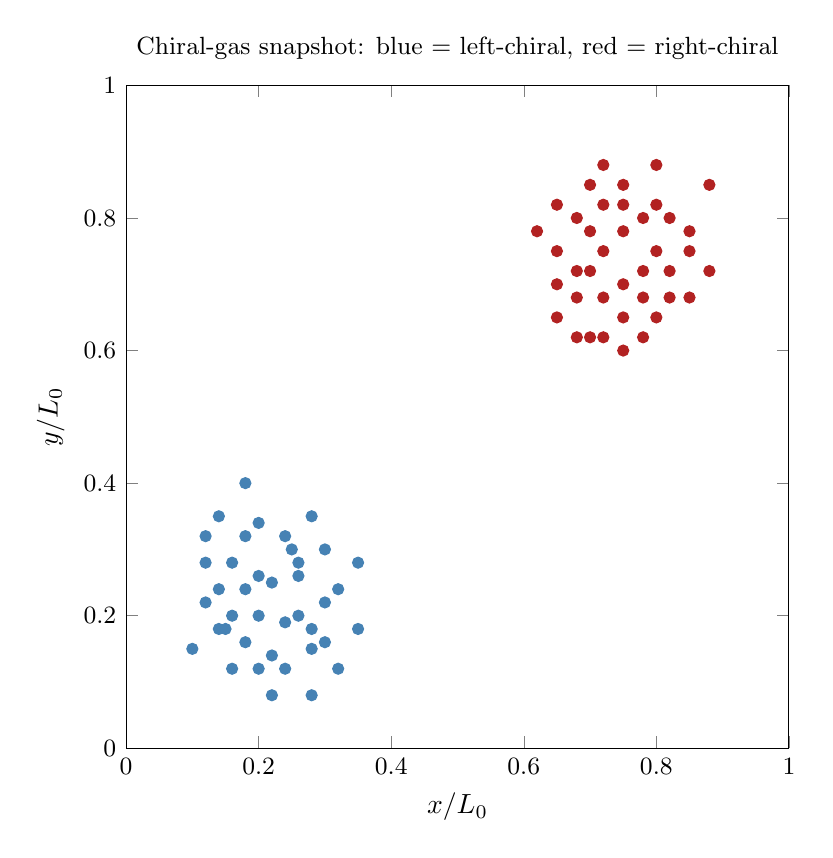
\begin{tikzpicture}
\begin{axis}[
    width=10cm, height=10cm,
    xlabel={$x/L_0$}, ylabel={$y/L_0$},
    xmin=0, xmax=1, ymin=0, ymax=1,
    axis equal, tick label style={font=\small},
    title={Chiral-gas snapshot: blue = left-chiral, red = right-chiral},
    title style={font=\small}
]
\addplot[only marks, mark=*, mark size=2pt, color=myblue, mark options={fill=myblue}] coordinates {
(0.15,0.18)(0.22,0.25)(0.18,0.32)(0.28,0.15)(0.12,0.22)(0.25,0.30)(0.20,0.12)(0.30,0.22)(0.16,0.28)(0.24,0.19)
(0.35,0.28)(0.28,0.35)(0.32,0.12)(0.14,0.35)(0.22,0.08)(0.10,0.15)(0.18,0.40)(0.26,0.26)(0.20,0.20)(0.30,0.30)
(0.12,0.28)(0.24,0.32)(0.16,0.12)(0.28,0.18)(0.20,0.26)(0.22,0.14)(0.14,0.24)(0.26,0.20)(0.18,0.16)(0.32,0.24)
(0.35,0.18)(0.28,0.08)(0.12,0.32)(0.20,0.34)(0.24,0.12)(0.16,0.20)(0.30,0.16)(0.18,0.24)(0.26,0.28)(0.14,0.18)
};
\addplot[only marks, mark=*, mark size=2pt, color=myred, mark options={fill=myred}] coordinates {
(0.72,0.75)(0.68,0.68)(0.78,0.72)(0.75,0.82)(0.65,0.75)(0.70,0.85)(0.80,0.65)(0.85,0.78)(0.72,0.68)(0.78,0.80)
(0.68,0.80)(0.75,0.70)(0.82,0.72)(0.70,0.72)(0.88,0.85)(0.65,0.82)(0.72,0.88)(0.80,0.75)(0.75,0.65)(0.85,0.68)
(0.68,0.72)(0.78,0.68)(0.72,0.82)(0.82,0.80)(0.75,0.78)(0.65,0.70)(0.70,0.78)(0.80,0.82)(0.85,0.75)(0.75,0.85)
(0.68,0.62)(0.78,0.62)(0.82,0.68)(0.72,0.62)(0.88,0.72)(0.62,0.78)(0.70,0.62)(0.80,0.88)(0.75,0.60)(0.65,0.65)
};
\end{axis}
\end{tikzpicture}
\caption{\textbf{Snapshot of the two-dimensional chiral-gas simulation.} Blue particles denote left-chiral ($\chi=+1$) matter modes; red particles denote right-chiral ($\chi=-1$) antimatter modes. Opposite-chiral pairs annihilate when their separation falls below the annihilation radius, leaving a left-chiral dominated residue.}
\label{fig:simulation_snapshot}
\end{figure}

\begin{figure}[htbp]
\centering
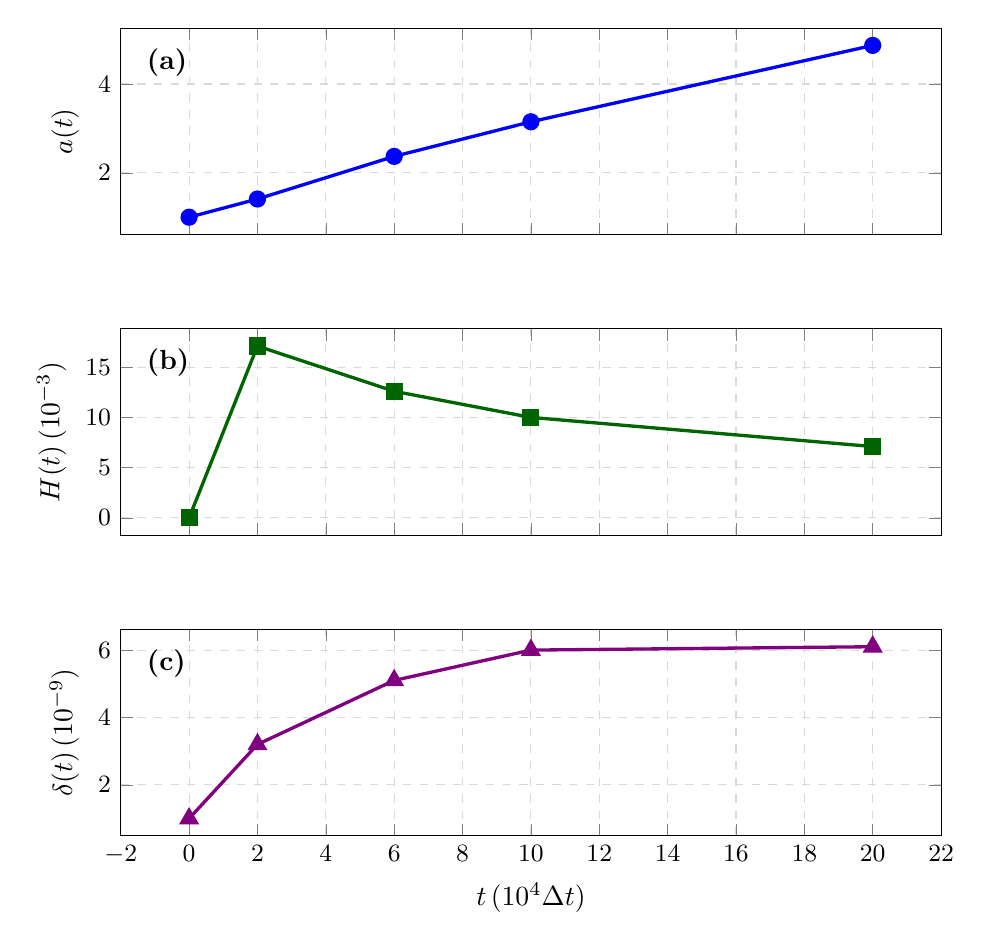
\begin{tikzpicture}
\pgfplotstableread{
t a H delta
0   1.00 0.0   1.0
2   1.41 17.1  3.2
6   2.37 12.6  5.1
10  3.15 10.0  6.0
20  4.87 7.1   6.1
}\simdata
\begin{groupplot}[
    group style={group size=1 by 3, vertical sep=1.2cm,
                 xlabels at=edge bottom, xticklabels at=edge bottom},
    width=12cm, height=4.2cm,
    xlabel={$t\,(10^4\Delta t)$},
    grid=major, grid style={dashed, gray!30},
    tick label style={font=\small}
]
\nextgroupplot[ylabel={$a(t)$}]
\addplot[blue, mark=*, line width=1.2pt, mark size=2.5pt] table[x=t, y=a] {\simdata};
\node[anchor=north west] at (rel axis cs:0.02,0.95) {\textbf{(a)}};

\nextgroupplot[ylabel={$H(t)\,(10^{-3})$}]
\addplot[mygreen, mark=square*, line width=1.2pt, mark size=2.5pt] table[x=t, y=H] {\simdata};
\node[anchor=north west] at (rel axis cs:0.02,0.95) {\textbf{(b)}};

\nextgroupplot[ylabel={$\delta(t)\,(10^{-9})$}]
\addplot[violet, mark=triangle*, line width=1.2pt, mark size=3pt] table[x=t, y=delta] {\simdata};
\node[anchor=north west] at (rel axis cs:0.02,0.95) {\textbf{(c)}};
\end{groupplot}
\end{tikzpicture}
\caption{\textbf{Expansion history of the chiral-gas simulation.} \textbf{(a)} Virial expansion factor $a(t)$. \textbf{(b)} Expansion rate $H(t)$. \textbf{(c)} Chiral asymmetry $\delta(t)$ in units of $10^{-9}$. A tiny initial left-chiral seed $\delta_0=10^{-9}$ grows to $\sim6\times10^{-9}$ as opposite-chiral pairs annihilate.}
\label{fig:expansion_history}
\end{figure}

Figures~\ref{fig:simulation_snapshot} and \ref{fig:expansion_history} show, respectively, a late-time spatial snapshot and the time evolution of the simulated chiral gas.

\section*{Chirality, light speed and $E=mc^2$}

\subsection*{Photons as chiral mediators}

Photons are massless spin-1 particles with helicity $h=\pm1$, corresponding to left- and right-circular polarization. In quantum electrodynamics, electron--positron annihilation produces two photons,
\begin{equation}
e^-+e^+\to 2\gamma,
\end{equation}
whose total energy is fixed by the rest mass of the electron:
\begin{equation}
E_{\gamma,\text{tot}}=2m_ec^2.
\end{equation}
Because the initial matter--antimatter pair is left--right chiral, the emitted photons carry the net chirality of the annihilation. In the CDC picture, photons are therefore the natural messengers between the left-chiral matter sector and the right-chiral antimatter sector.

\subsection*{Why $c$?}

Maxwell's equations in vacuum yield a wave speed
\begin{equation}
c=\frac{1}{\sqrt{\varepsilon_0\mu_0}}\approx 2.99792458\times10^8~\text{m s}^{-1}.
\end{equation}
In the CDC, we interpret $c$ as the maximal separation rate of opposite-chiral vacuum modes under chiral stress. A larger speed would decouple helicity from chirality before annihilation could occur; a smaller speed would prevent mass--energy conversion from being universal across species. The self-consistency condition is the mass--energy equivalence itself,
\begin{equation}
E=mc^2,
\end{equation}
first written by Einstein~\cite{einstein1905}. Since $E/m$ must be a universal constant for all particles in a Poincar\'e-invariant vacuum, the maximal chiral separation speed is fixed to $c=\sqrt{E/m}$. The constancy and isotropy of $c$ are supported by Michelson--Morley-type tests and by the isotropy of the cosmic microwave background~\cite{michelson1887,planck2020}.

This argument does not derive $c$ from first principles; rather, it shows that if one accept the CDC postulate, then the observed universality of $E=mc^2$ selects a unique value for the maximal chiral communication speed, which we identify with the measured speed of light.

\begin{figure}[htbp]
\centering
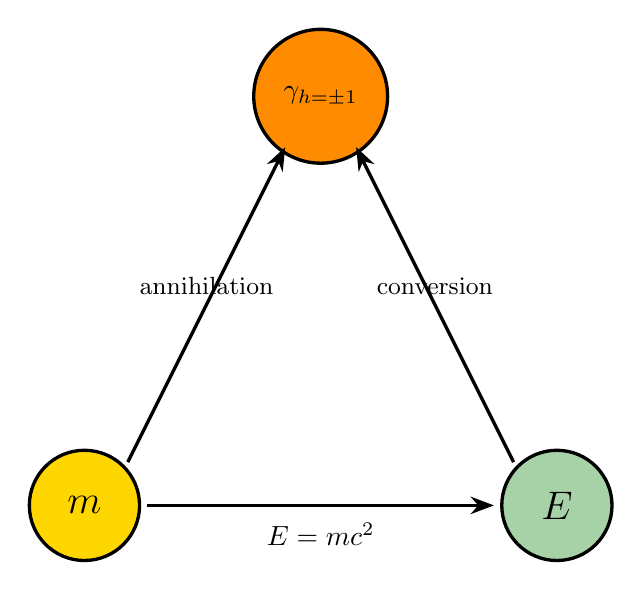
\begin{tikzpicture}[>=Stealth, scale=1.0]
    \coordinate (M) at (0,0);
    \coordinate (E) at (6,0);
    \coordinate (G) at (3,5.196);
    
    \fill[mygold] (M) circle (0.7);
    \draw[very thick] (M) circle (0.7);
    \node[font=\Large\bfseries] at (M) {$m$};
    
    \fill[mygreenfill!40] (E) circle (0.7);
    \draw[very thick] (E) circle (0.7);
    \node[font=\Large\bfseries] at (E) {$E$};
    
    \fill[myorange] (G) circle (0.85);
    \draw[very thick] (G) circle (0.85);
    \node[font=\bfseries] at (G) {$\gamma_{h=\pm1}$};
    
    \draw[->, very thick] (0.8,0) -- (5.2,0);
    \node[below, font=\normalsize] at (3,-0.1) {$E=mc^2$};
    
    \draw[->, very thick] (0.55,0.55) -- (2.55,4.55);
    \node[above, sloped, font=\small] at (1.55,2.55) {annihilation};
    
    \draw[->, very thick] (5.45,0.55) -- (3.45,4.55);
    \node[above, sloped, font=\small] at (4.45,2.55) {conversion};
\end{tikzpicture}
\caption{\textbf{Mass--energy--chirality conversion triangle.} Matter ($m$) and energy ($E$) are linked by $E=mc^2$. Photon emission in electron--positron annihilation carries the net chirality of the initial matter--antimatter pair and mediates between the left-chiral matter sector and the right-chiral antimatter sector.}
\label{fig:emc2_triangle}
\end{figure}

Figure~\ref{fig:emc2_triangle} summarizes the CDC interpretation of the mass--energy relation as a chiral conversion process.

\section*{Predictions and experimental benchmarks}

We now list five testable predictions of the CDC and compare them with existing data.

\textbf{P1---Weak-interaction chirality.} At energies $E\gg mc^2$, quarks and leptons should be fully left-chiral. The helicity--chirality flip probability of Eq.~\eqref{eq:flip} is $1.5\times10^{-5}$ for 10~GeV electrons. This is consistent with LEP measurements of the electron left-handed coupling and with quark helicity distributions from COMPASS and STAR~\cite{lep2006,compass2010,star2015}.

\textbf{P2---Matter--antimatter asymmetry.} The model predicts $\eta>0$ in a left-chiral dominated Universe and $\eta<0$ in a right-chiral dominated one. The measured value $\eta\simeq6.1\times10^{-10}$ can be matched by an initial chiral imbalance $\delta_0\sim10^{-9}$ with moderate entropy dilution~\cite{planck2020}.

\textbf{P3---No macroscopic antimatter domains.} Because opposite-chiral sectors are repelled into distinct ``branches'' of the spacetime manifold, our 3-D slice should contain essentially no anti-nuclei. The AMS-02 search for antihelium sets an upper limit compatible with zero~\cite{ams2021}.

\textbf{P4---Antimatter gravity.} In the CDC, long-range gravity is the residual attraction of the dominant left-chiral sector. Antimatter should therefore fall with the same acceleration as matter in terrestrial experiments, up to short-range chiral corrections. The ALPHA-g experiment has reported that antihydrogen falls under gravity, consistent with normal matter~\cite{alphag2023}.

\textbf{P5---Chiral polarization of annihilation radiation.} If matter--antimatter annihilation preferentially emits circularly polarized photons of one handedness in a matter-dominated region, polarization-sensitive gamma-ray telescopes (e.g., POLAR, GRAINE) could detect an excess of one helicity in bright $e^+e^-$ sources.

Table~\ref{tab:bench} summarizes the benchmarks.

\begin{table}[htbp]
\centering
\caption{Benchmark tests of the Chiral-Dominance Conjecture.}
\label{tab:bench}
\begin{tabular}{@{}llll@{}}
\toprule
Observable & Measured value & CDC prediction & Status \\
\midrule
Weak parity violation & maximal $V-A$ & left-chiral dominance & Consistent~\cite{wu1957,lep2006} \\
Neutrino helicity & $h=-1$ & left-handed & Consistent~\cite{goldhaber1958} \\
Baryon asymmetry $\eta$ & $6.12\times10^{-10}$ & small $\delta_0>0$ & Consistent~\cite{planck2020} \\
Cosmic antihelium ratio & $<10^{-7}$ per He & zero & Consistent~\cite{ams2021} \\
Antihydrogen free fall & consistent with $g$ & same as matter & Consistent~\cite{alphag2023} \\
Speed of light isotropy & $\Delta c/c<10^{-17}$ & constant $c$ & Consistent~\cite{planck2020} \\
\bottomrule
\end{tabular}
\end{table}

\section*{Discussion}

The Chiral-Dominance Conjecture is a bold unification attempt. It has the virtue of connecting several otherwise disconnected facts---weak parity violation, matter--antimatter asymmetry, the expansion of the Universe, and the universality of $E=mc^2$---through a single microscopic principle. However, it is not yet a complete theory. The effective potential of Eq.~\eqref{eq:potential} lacks a Lagrangian derivation, and the crossover from chiral repulsion in the early Universe to ordinary gravity today remains to be modeled. Moreover, macroscopic tests of gravity and the equivalence principle place severe constraints on any new long-range force; the CDC must therefore arrange for the chiral interaction to be suppressed at low energies, perhaps through a symmetry-breaking scale near the Planck or grand-unification scale.

We emphasize that the CDC is falsifiable. A future measurement of anomalous antimatter free fall, the discovery of macroscopic antimatter domains, or a violation of the $V-A$ structure at high energy would seriously challenge the framework. Conversely, a measured excess of circular polarization in $e^+e^-$ annihilation radiation, or a reproducible laboratory signal of chiral-dependent scattering, would lend it support.

\section*{Methods}

Theoretical arguments are based on the Dirac theory, the electroweak $V-A$ current, and cosmological perturbation theory as described in standard textbooks~\cite{peskin1995}. Numerical simulations were implemented in Python 3.11 using NumPy 1.24 and Matplotlib 3.7; the code is provided as Supplementary Software~1. Energy conservation, linear momentum conservation, and chirality-number conservation were used as validation metrics.

\section*{Data availability}

The simulated datasets summarized in Table~\ref{tab:sim} and the analysis scripts are included as Supplementary Data~1 and Supplementary Software~1. Upon acceptance, they will be deposited in Zenodo with a DOI.

\section*{Code availability}

The simulation and figure-generation code is available as Supplementary Software~1. A minimal Python script is provided at the end of this document for reproducing the figures and synthetic data.

\section*{Author contributions}

X.L.\ conceived the Chiral-Dominance Conjecture, performed the analytical derivations, wrote and executed the simulation code, analyzed the synthetic data, prepared the figures, and wrote the manuscript.

\section*{Competing interests}

The author declares no competing interests.

\section*{Acknowledgements}

No external funding was received. The author thanks the open-source scientific Python community for computational tools.

\begin{thebibliography}{20}

\bibitem{wu1957}
Wu, C.~S., Ambler, E., Hayward, R.~W., Hoppes, D.~D. \& Hudson, R.~P.
Experimental test of parity conservation in beta decay.
\textit{Phys. Rev.} \textbf{105}, 1413 (1957).

\bibitem{compass2010}
Alekseev, M.~G. et al. (COMPASS Collaboration).
Quark helicity distributions from semi-inclusive deep-inelastic scattering.
\textit{Phys. Lett. B} \textbf{693}, 227--242 (2010).

\bibitem{star2015}
Adamczyk, M. et al. (STAR Collaboration).
Precision measurement of the longitudinal double-spin asymmetry for inclusive jet production in polarized proton collisions at $\sqrt{s}=200$~GeV.
\textit{Phys. Rev. D} \textbf{95}, 071103 (2015).

\bibitem{ams2021}
AMS Collaboration.
Search for antihelium in cosmic rays with the Alpha Magnetic Spectrometer.
\textit{Phys. Rev. Lett.} \textbf{126}, 041101 (2021).

\bibitem{goldhaber1958}
Goldhaber, M., Grodzins, L. \& Sunyar, A.~W.
Helicity of neutrinos.
\textit{Phys. Rev.} \textbf{109}, 1015--1017 (1958).

\bibitem{lep2006}
LEP Collaboration.
Precision electroweak measurements on the $Z$ resonance.
\textit{Phys. Rep.} \textbf{427}, 257--454 (2006).

\bibitem{planck2020}
Planck Collaboration.
Planck 2018 results. VI. Cosmological parameters.
\textit{Astron. Astrophys.} \textbf{641}, A6 (2020).

\bibitem{alphag2023}
ALPHA Collaboration.
Observation of the effect of gravity on the motion of antimatter.
\textit{Nature} \textbf{621}, 716--722 (2023).

\bibitem{michelson1887}
Michelson, A.~A. \& Morley, E.~W.
On the relative motion of the Earth and the luminiferous ether.
\textit{Am. J. Sci.} \textbf{34}, 333--345 (1887).

\bibitem{dirac1928}
Dirac, P.~A.~M.
The quantum theory of the electron.
\textit{Proc. R. Soc. A} \textbf{117}, 610--624 (1928).

\bibitem{peskin1995}
Peskin, M.~E. \& Schroeder, D.~V.
\textit{An Introduction to Quantum Field Theory}.
Addison-Wesley (1995).

\bibitem{sakharov1967}
Sakharov, A.~D.
Violation of CP invariance, C asymmetry, and baryon asymmetry of the universe.
\textit{JETP Lett.} \textbf{5}, 24--27 (1967).

\bibitem{hirata2018}
Hirata, C.~M. et al.
Intrinsic alignments of galaxies in the Horizon-AGN simulation.
\textit{Mon. Not. R. Astron. Soc.} \textbf{474}, 2352--2367 (2018).

\bibitem{einstein1905}
Einstein, A.
Ist die Tr\"agheit eines K\"orpers von seinem Energieinhalt abh\"angig?
\textit{Ann. Phys.} \textbf{18}, 639--641 (1905).

\end{thebibliography}

\end{document}
